\documentclass[border=0pt,10pt]{standalone}
\usepackage[T1]{fontenc}
\usepackage{lmodern}
\usepackage{pgfplots}
\pgfplotsset{compat=1.17}
\usepgfplotslibrary{groupplots}
\usepackage{xcolor}
\definecolor{oi-blue}{HTML}{0072B2}
\definecolor{oi-vermillion}{HTML}{D55E00}
\definecolor{oi-green}{HTML}{009E73}
\definecolor{oi-purple}{HTML}{CC79A7}
\definecolor{oi-black}{HTML}{000000}
% semantic_sha256: bd2a953e6fdeba82f892112e77e569b479863bd0d1672a21f119ca1f80c333bc
\begin{document}
\begin{minipage}{181.86mm}
\centering
{\bfseries\fontsize{10}{12}\selectfont PP-U-ARPLS | D1 | source\_fit}\\[2mm]
{\fontsize{8}{10}\selectfont planned=108, monitored=105, missing-history=3, status=partial\_history\_coverage}\\[3mm]
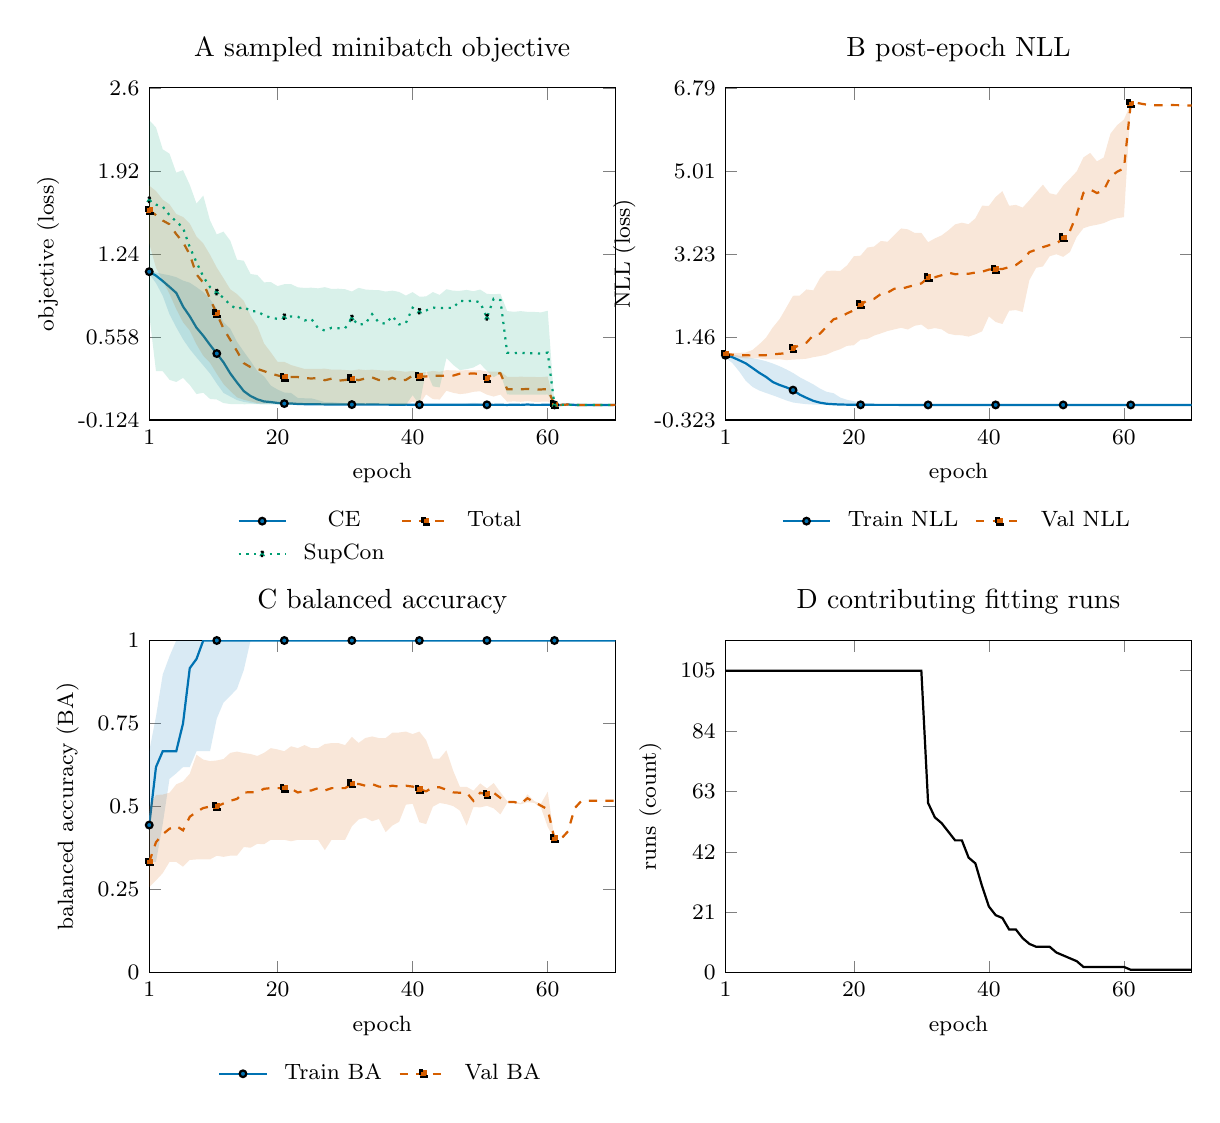
\begin{tikzpicture}
\begin{groupplot}[group style={group size=2 by 2, horizontal sep=14mm, vertical sep=28mm}]
\nextgroupplot[width=75mm, height=58mm, title={A sampled minibatch objective}, xlabel={epoch}, ylabel={objective (loss)}, xmin=1, xmax=70, xtick={1,20,40,60}, ymin=-0.12394953787326812, ymax=2.6029402953386307, ytick={-0.12394953787326812,0.55777292042970661,1.2394953787326815,1.9212178370356559,2.6029402953386307}, yticklabels={-0.124,0.558,1.24,1.92,2.6}, tick label style={font=\fontsize{8}{9}\selectfont, text=black}, label style={font=\fontsize{8}{9}\selectfont, text=black}, title style={font=\fontsize{10}{11}\selectfont, text=black}, legend style={at={(0.5,-0.24)},anchor=north,draw=none,fill=none,font=\fontsize{8}{9}\selectfont,row sep=1pt,column sep=4pt,legend columns=2}]
\addplot[fill=oi-blue,opacity=0.15,draw=none,forget plot] coordinates {(1,1.0751751422882081) (2,1.0001464128494262) (3,0.89576182663440707) (4,0.7444569885730743) (5,0.63765119016170502) (6,0.53925139605998995) (7,0.4584095597267151) (8,0.38993119746446608) (9,0.32463063746690751) (10,0.25783946588635442) (11,0.17497241050004958) (12,0.098851083032786849) (13,0.06885981243103742) (14,0.039865057636052373) (15,0.024784019310027362) (16,0.016681473562493922) (17,0.0082081826170906421) (18,0.0068278007267508654) (19,0.0069937683874741197) (20,0.0045857186720240865) (21,0.0032832893193699419) (22,0.0029363492270931602) (23,0.0023833303712308407) (24,0.0023480035568354653) (25,0.0024675042310263961) (26,0.0015595525459502825) (27,0.0013444162948871962) (28,0.0011463345377705993) (29,0.00080586900148773568) (30,0.0011814441793831065) (31,0.001141304394695908) (32,0.0014770369714824482) (33,0.0013395222718827426) (34,0.0011939887723201538) (35,0.001189556811368675) (36,0.0010431839618831873) (37,0.00094260025289258917) (38,0.00097571949736448001) (39,0.00084075220574959537) (40,0.00086336462409235541) (41,0.00077054061985109006) (42,0.00085164377815090116) (43,0.00072020525258267301) (44,0.00088374697807012124) (45,0.0011629860811808613) (46,0.00072660002479096875) (47,0.00065462177735753357) (48,0.00054602532982244161) (49,0.00098095993162132804) (50,0.0007876643125200645) (51,0.00042892909550573677) (52,0.00038224769123189616) (53,0.00092101624904898931) (54,0.00015065754018905864) (55,0.0012645662814975366) (56,0.00012790017153747614) (57,0.0015099590301360876) (58,0.00035827537212753671) (59,0.00043548257774546074) (60,0.00070373728121921888) (61,0.00010472725807630923) (62,0.00033481124046375044) (63,0.0034069789871864486) (64,0.00037326101528378786) (65,6.539318201248534e-05) (66,9.6188236000216421e-05) (67,0.00011996501416433603) (68,0.00011204219026694773) (69,0.00015497880849579815) (70,0.00041266055200139817) (70,0.00041266055200139817) (69,0.00015497880849579815) (68,0.00011204219026694773) (67,0.00011996501416433603) (66,9.6188236000216421e-05) (65,6.539318201248534e-05) (64,0.00037326101528378786) (63,0.0034069789871864486) (62,0.00033481124046375044) (61,0.00010472725807630923) (60,0.0016155522829649272) (59,0.00084513870872342527) (58,0.00053398498712340368) (57,0.005423023452658526) (56,0.00061498999657487734) (55,0.0036267563476940269) (54,0.00019387376528356981) (53,0.0073519652254617554) (52,0.0010634947480866687) (51,0.001435413218132453) (50,0.012270128398085953) (49,0.017950401520647585) (48,0.010082005183357983) (47,0.0060449568220064991) (46,0.0046997016637760677) (45,0.0029808888866682537) (44,0.0026891056768363342) (43,0.0026572762755677102) (42,0.0029505279031582163) (41,0.0033652030542725701) (40,0.0038021714426577091) (39,0.005850291595970703) (38,0.0048531909415032715) (37,0.0073035393783357008) (36,0.006414480814783019) (35,0.0076320834414218552) (34,0.011534818331710994) (33,0.0076555000094231202) (32,0.012612795640598055) (31,0.0072473311854992098) (30,0.013349015722633351) (29,0.018484964244998993) (28,0.023422124213539109) (27,0.022409857739694429) (26,0.039431293215602729) (25,0.054193515307270033) (24,0.054857742972672097) (23,0.057088609971106062) (22,0.0980186963453889) (21,0.10192210003733645) (20,0.12608747631311418) (19,0.15917594209313407) (18,0.23450993821024899) (17,0.27846416682004954) (16,0.36040988117456441) (15,0.43748551309108741) (14,0.51775114536285438) (13,0.62537453174591073) (12,0.67992863655090341) (11,0.79098474681377418) (10,0.86786761283874514) (9,0.92697870433330554) (8,0.96653379499912262) (7,1.0032733112573624) (6,1.021192193031311) (5,1.0490074396133422) (4,1.0643175840377808) (3,1.0746995806694031) (2,1.0871059358119965) (1,1.1046436965465545)};
\addplot[color=oi-blue, mark=*, mark options={draw=black}, mark repeat=10, mark size=1.2pt, solid, line width=0.8pt] coordinates {(1,1.0938965678215027) (2,1.0611922442913055) (3,1.0170543640851974) (4,0.96924863755702972) (5,0.91961738467216492) (6,0.80841408669948578) (7,0.72771647572517395) (8,0.63384526968002319) (9,0.5683063268661499) (10,0.49286991357803345) (11,0.42185812443494797) (12,0.34959384799003601) (13,0.25854894518852234) (14,0.18414797633886337) (15,0.11343817040324211) (16,0.073157343082129955) (17,0.046260139904916286) (18,0.028707623481750488) (19,0.023488310631364584) (20,0.01635767740663141) (21,0.011374699475709349) (22,0.011968933045864105) (23,0.0078679341822862625) (24,0.0063797099282965064) (25,0.0059795855777338147) (26,0.005040560761699453) (27,0.0043701088579837233) (28,0.003807687375228852) (29,0.003438406070927158) (30,0.0033792947942856699) (31,0.0029992721320013516) (32,0.0033302520314464346) (33,0.0026436582993483171) (34,0.0032855552271939814) (35,0.0027225108788115904) (36,0.0025020290559041314) (37,0.0023264037081389688) (38,0.001931823200720828) (39,0.0024490567921020556) (40,0.0021628655667882413) (41,0.0014776253919990268) (42,0.0013247674578451551) (43,0.0014138157130219042) (44,0.0012531617030617781) (45,0.0023880717544670915) (46,0.0012865544704254717) (47,0.0011666787468129769) (48,0.00099891125864814967) (49,0.0017362001235596836) (50,0.0022930889390408993) (51,0.00099955981386301573) (52,0.00059613804842229001) (53,0.001202932427986525) (54,0.00017226565273631422) (55,0.0024456613145957817) (56,0.00037144508405617671) (57,0.003466491241397307) (58,0.00044613017962547019) (59,0.00064031064323444298) (60,0.001159644782092073) (61,0.00010472725807630923) (62,0.00033481124046375044) (63,0.0034069789871864486) (64,0.00037326101528378786) (65,6.539318201248534e-05) (66,9.6188236000216421e-05) (67,0.00011996501416433603) (68,0.00011204219026694773) (69,0.00015497880849579815) (70,0.00041266055200139817)};
\addlegendentry{CE}
\addplot[fill=oi-vermillion,opacity=0.15,draw=none,forget plot] coordinates {(1,1.3249642968177795) (2,1.1262446284294128) (3,1.0188517719507217) (4,0.91261540055274959) (5,0.78721242249011991) (6,0.67910709679126735) (7,0.610717436671257) (8,0.49679002165794373) (9,0.40388129800558092) (10,0.34603045508265495) (11,0.25543198063969613) (12,0.17153045609593393) (13,0.1141041973605752) (14,0.062400899920612575) (15,0.042684088274836537) (16,0.02911768201738596) (17,0.015457209199666977) (18,0.011734683043323459) (19,0.013676064337778371) (20,0.0090563156176358458) (21,0.0053100020624697207) (22,0.0057401563404710036) (23,0.0049962184159085153) (24,0.0049274995108135045) (25,0.0069186441134661452) (26,0.0033233526657568289) (27,0.0027660032093990592) (28,0.0023342769942246381) (29,0.002038792136590928) (30,0.0023139682976761832) (31,0.0033689237781800332) (32,0.0030904859915608547) (33,0.0032208881544647742) (34,0.0045660168310860186) (35,0.0045084681405569427) (36,0.0035205225649406202) (37,0.0049427634501626027) (38,0.0025600681008654648) (39,0.0022742511311662386) (40,0.027810867864172927) (41,0.0013473072152919486) (42,0.086857741590938536) (43,0.047370437203790076) (44,0.044103449568501686) (45,0.11648853179067374) (46,0.099698537259246225) (47,0.089035341255657846) (48,0.094475634745322168) (49,0.1078081794839818) (50,0.11250596689060333) (51,0.084699120594450505) (52,0.068660953705693833) (53,0.085325557042233421) (54,0.025928425329948369) (55,0.029165420209210424) (56,0.025823323527765753) (57,0.030918025256505645) (58,0.025859217121069381) (59,0.026184535088304983) (60,0.027410628743746203) (61,0.00020098280219826847) (62,0.00043067339720437303) (63,0.0035946441275882535) (64,0.0004155862898187479) (65,0.00011712405466823839) (66,0.00011045758628824842) (67,0.00017410987129551359) (68,0.0001797232725948561) (69,0.00018119292963092448) (70,0.00044987172668697895) (70,0.00044987172668697895) (69,0.00018119292963092448) (68,0.0001797232725948561) (67,0.00017410987129551359) (66,0.00011045758628824842) (65,0.00011712405466823839) (64,0.0004155862898187479) (63,0.0035946441275882535) (62,0.00043067339720437303) (61,0.00020098280219826847) (60,0.23268876499023464) (59,0.22834027542694457) (58,0.22958212210887724) (57,0.23080089614140889) (56,0.23169069473387935) (55,0.23068667818824906) (54,0.23140757476157889) (53,0.27479077577590943) (52,0.2732361316680908) (51,0.27479016780853271) (50,0.28590410947799683) (49,0.28321210891008375) (48,0.2856847420334816) (47,0.28260315805673597) (46,0.28280476331710813) (45,0.28599724918603897) (44,0.27257292568683622) (43,0.27929177284240725) (42,0.26949428617954252) (41,0.26951197907328606) (40,0.28007268905639648) (39,0.27224126309156421) (38,0.27928496077656745) (37,0.28363253623247148) (36,0.28161563724279404) (35,0.28537502512335777) (34,0.28971704393625258) (33,0.28638323917984965) (32,0.29165083095431332) (31,0.28266281485557554) (30,0.28694146424531936) (29,0.29044647812843322) (28,0.28993669599294664) (27,0.2978478148579598) (26,0.29577432423830036) (25,0.29525562673807143) (24,0.29568358212709428) (23,0.31139438748359688) (22,0.32731559798121462) (21,0.35384554862976103) (20,0.35409762263298045) (19,0.43158764392137555) (18,0.50478600114583971) (17,0.64623529016971626) (16,0.7322103738784792) (15,0.85473041832447072) (14,0.90980415344238286) (13,0.94921707808971423) (12,1.0398982971906663) (11,1.1277226388454438) (10,1.2329729139804841) (9,1.3252055823802948) (8,1.382508671283722) (7,1.4888403475284577) (6,1.5430396139621736) (5,1.5669931590557098) (4,1.6465878367424014) (3,1.6858897149562835) (2,1.7557203412055971) (1,1.8002076327800751)};
\addplot[color=oi-vermillion, mark=square*, mark options={draw=black}, mark repeat=10, mark size=1.2pt, dashed, line width=0.8pt] coordinates {(1,1.5962285697460175) (2,1.5585801303386688) (3,1.5140310227870941) (4,1.483142077922821) (5,1.4023369550704956) (6,1.3359303772449493) (7,1.2350929379463196) (8,1.0711155831813812) (9,1.0037743151187897) (10,0.87163890898227692) (11,0.7482462078332901) (12,0.62669160962104797) (13,0.53460299968719482) (14,0.44128061085939407) (15,0.34289053827524185) (16,0.31028401106595993) (17,0.29608564078807831) (18,0.2773863896727562) (19,0.25709185004234314) (20,0.24238933250308037) (21,0.22826282307505608) (22,0.23016717284917831) (23,0.22917546704411507) (24,0.22018727287650108) (25,0.21725822240114212) (26,0.22057866305112839) (27,0.20268189162015915) (28,0.21562528237700462) (29,0.19897861033678055) (30,0.20462169870734215) (31,0.21386077627539635) (32,0.20351622439920902) (33,0.21728415042161942) (34,0.22596123069524765) (35,0.20447158627212048) (36,0.20208263769745827) (37,0.22320001199841499) (38,0.19956663809716702) (39,0.20572640560567379) (40,0.24033530429005623) (41,0.23236260935664177) (42,0.2339496947824955) (43,0.24087739363312721) (44,0.23971511423587799) (45,0.24103308282792568) (46,0.24062142334878445) (47,0.25691301375627518) (48,0.25537753850221634) (49,0.2589108794927597) (50,0.25281432271003723) (51,0.2156639602035284) (52,0.26303055882453918) (53,0.25935514643788338) (54,0.12866800004576362) (55,0.12992604919872974) (56,0.12875700913082255) (57,0.13085946069895726) (58,0.1277206696149733) (59,0.12726240525762478) (60,0.13004969686699042) (61,0.00020098280219826847) (62,0.00043067339720437303) (63,0.0035946441275882535) (64,0.0004155862898187479) (65,0.00011712405466823839) (66,0.00011045758628824842) (67,0.00017410987129551359) (68,0.0001797232725948561) (69,0.00018119292963092448) (70,0.00044987172668697895)};
\addlegendentry{Total}
\addplot[fill=oi-green,opacity=0.15,draw=none,forget plot] coordinates {(1,0.74319007396698) (2,0.27737919315695764) (3,0.27658624872565268) (4,0.20673046410083773) (5,0.18834301517345015) (6,0.22168716844171285) (7,0.16465893164277079) (8,0.08898680806159974) (9,0.10037097334861755) (10,0.04924497606698424) (11,0.044627142092213037) (12,0.015266275417525323) (13,0.0076688828296028076) (14,0.0068145216908305885) (15,0.0056297660106793051) (16,0.0057076990648056384) (17,0.0063679456710815435) (18,0.0041920602787286045) (19,0.0048161388956941666) (20,0.0042927145492285494) (21,0.0041676282242406161) (22,0.0022357583220582455) (23,0.0024798631791782101) (24,0.002605056797619909) (25,0.0023668766138143838) (26,0.0015057147014886142) (27,0.0014933824757463298) (28,0.00132632254390046) (29,0.0010735153977293522) (30,0.0012776493473211302) (31,0.0021746098937001079) (32,0.0049040794423490302) (33,0.0014350534198456445) (34,0.0016985118912998588) (35,0.0019202233015676029) (36,0.0017072260525310412) (37,0.0017744034659699542) (38,0.0007953435182571412) (39,0.0012879014044301588) (40,0.080463176965713576) (41,0.0015921175479888918) (42,0.28227501511719311) (43,0.15263771417376124) (44,0.14389568865735788) (45,0.38405522778630258) (46,0.32859741002321241) (47,0.28602373004032416) (48,0.29380055070068922) (49,0.30741263031977728) (50,0.33761460484383865) (51,0.27990255504937522) (52,0.22743496894836426) (53,0.26025009304285052) (54,0.085925889015197765) (55,0.085128875076770791) (56,0.085651412608285682) (57,0.084983330966679205) (58,0.085003134612361475) (59,0.084464648365974435) (60,0.085983583331926641) (61,0.00032085180646390654) (62,0.00031954051519278437) (63,0.00062555076146963984) (64,0.00014108419509284431) (65,0.00017243623733520508) (66,4.7564507895003771e-05) (67,0.00018048286983685102) (68,0.00022560358047485352) (69,8.7380409240722656e-05) (70,0.0001240372694155667) (70,0.0001240372694155667) (69,8.7380409240722656e-05) (68,0.00022560358047485352) (67,0.00018048286983685102) (66,4.7564507895003771e-05) (65,0.00017243623733520508) (64,0.00014108419509284431) (63,0.00062555076146963984) (62,0.00031954051519278437) (61,0.00032085180646390654) (60,0.77328338325032753) (59,0.75968258678913114) (58,0.76349374949977578) (57,0.76430304646510194) (56,0.77025236189388124) (55,0.76474033147096632) (54,0.77071230411529545) (53,0.91256102919578552) (52,0.90860352218151097) (51,0.91181749850511551) (50,0.94706117808818813) (49,0.93350870311260226) (48,0.94406532347202299) (47,0.936862176656723) (46,0.93772093206644058) (45,0.94988410770893095) (44,0.90316885113716128) (43,0.92658491432666779) (42,0.8908217072486877) (41,0.88885014057159428) (40,0.92629233300685887) (39,0.8978072434663773) (38,0.92779683321714401) (37,0.93834410160779957) (36,0.93086308985948563) (35,0.94250715523958206) (34,0.94378856718540194) (33,0.9474599108099937) (32,0.96154628098011019) (31,0.93103618919849396) (30,0.94977929294109342) (29,0.95419534444808962) (28,0.95215329825878148) (27,0.96681752204895033) (26,0.95724137127399445) (25,0.96246630549430856) (24,0.9608551412820816) (23,0.96527737379074097) (22,0.9920280188322067) (21,0.99110339283943183) (20,0.97560563683509827) (19,1.00890389084816) (18,1.006544440984726) (17,1.0668049693107609) (16,1.0746151655912399) (15,1.1840175271034241) (14,1.1924257576465609) (13,1.3484916150569923) (12,1.4227532267570506) (11,1.4002747595310212) (10,1.5147262513637545) (9,1.7186142027378082) (8,1.6528866410255434) (7,1.806973844766617) (6,1.9276175856590272) (5,1.9072025120258334) (4,2.0628433763980869) (3,2.0983379185199738) (2,2.278677606582642) (1,2.3377814531326297)};
\addplot[color=oi-green, mark=triangle*, mark options={draw=black}, mark repeat=10, mark size=1.2pt, dotted, line width=0.8pt] coordinates {(1,1.6797602474689484) (2,1.6443949639797211) (3,1.6285289525985718) (4,1.5579173862934113) (5,1.5056088864803314) (6,1.455014705657959) (7,1.2950012981891632) (8,1.1709778010845184) (9,1.0534668415784836) (10,0.96689069271087646) (11,0.92289553582668304) (12,0.8788619339466095) (13,0.8201974481344223) (14,0.78677816689014435) (15,0.80643333494663239) (16,0.76891031861305237) (17,0.76790300011634827) (18,0.73510456085205078) (19,0.71648575365543365) (20,0.7068016529083252) (21,0.72039434313774109) (22,0.7265532910823822) (23,0.72408144176006317) (24,0.69314602017402649) (25,0.7063889354467392) (26,0.63041503727436066) (27,0.61055240035057068) (28,0.63354384899139404) (29,0.62991231679916382) (30,0.62996974587440491) (31,0.71023207902908325) (32,0.65751300752162933) (33,0.66753922402858734) (34,0.74555788934230804) (35,0.67618335783481598) (36,0.66697578132152557) (37,0.728859543800354) (38,0.66113229840993881) (39,0.6727503165602684) (40,0.79809434711933136) (41,0.76526294648647308) (42,0.77598764002323151) (43,0.79928629100322723) (44,0.79541869461536407) (45,0.79654569178819656) (46,0.79720374196767807) (47,0.85476914048194885) (48,0.84980933368206024) (49,0.85724887251853943) (50,0.84127430617809296) (51,0.71591100841760635) (52,0.87251228094100952) (53,0.86050733178853989) (54,0.42831909656524658) (55,0.42493460327386856) (56,0.42795188725108346) (57,0.42464318871589057) (58,0.4242484420560686) (59,0.4220736175775528) (60,0.42963348329112705) (61,0.00032085180646390654) (62,0.00031954051519278437) (63,0.00062555076146963984) (64,0.00014108419509284431) (65,0.00017243623733520508) (66,4.7564507895003771e-05) (67,0.00018048286983685102) (68,0.00022560358047485352) (69,8.7380409240722656e-05) (70,0.0001240372694155667)};
\addlegendentry{SupCon}
\nextgroupplot[width=75mm, height=58mm, title={B post-epoch NLL}, xlabel={epoch}, ylabel={NLL (loss)}, xmin=1, xmax=70, xtick={1,20,40,60}, ymin=-0.32335245129600143, ymax=6.7904014772160295, ytick={-0.32335245129600143,1.4550860308320064,3.2335245129600141,5.0119629950880213,6.7904014772160295}, yticklabels={-0.323,1.46,3.23,5.01,6.79}, tick label style={font=\fontsize{8}{9}\selectfont, text=black}, label style={font=\fontsize{8}{9}\selectfont, text=black}, title style={font=\fontsize{10}{11}\selectfont, text=black}, legend style={at={(0.5,-0.24)},anchor=north,draw=none,fill=none,font=\fontsize{8}{9}\selectfont,row sep=1pt,column sep=4pt,legend columns=2}]
\addplot[fill=oi-blue,opacity=0.15,draw=none,forget plot] coordinates {(1,1.0117899551588212) (2,0.89979506526276365) (3,0.72418429226682701) (4,0.51731843183092674) (5,0.3864426736126596) (6,0.3084902579749903) (7,0.25656435847516273) (8,0.20600035278850926) (9,0.15317544713253528) (10,0.096525410136719836) (11,0.052220191368787243) (12,0.031858657798423784) (13,0.016345928223691832) (14,0.0080361268068627357) (15,0.0055503419613955026) (16,0.0031069234868207249) (17,0.0016362563708842036) (18,0.0013405983598634705) (19,0.0009358752298943352) (20,0.0007936160171724512) (21,0.00060813127966710776) (22,0.00040382612035017772) (23,0.00036637828023304976) (24,0.00033559901199250878) (25,0.00027685288186847246) (26,0.00025691076992185994) (27,0.00022494443049275636) (28,0.00020075220598170484) (29,0.00018666730391863595) (30,0.00017050223343079274) (31,0.0002161487160325175) (32,0.00023340066447616309) (33,0.00022098979556727853) (34,0.00022723569075364363) (35,0.0002036393359744824) (36,0.00019426622630606865) (37,0.0001688593622109787) (38,0.00017511728467822497) (39,0.00017018758809384533) (40,0.00013273459838533054) (41,0.00012142157280184554) (42,0.0001487959161531378) (43,8.9657586641897155e-05) (44,8.9530739447372194e-05) (45,0.00018983217828255831) (46,0.00017234157086497542) (47,9.1657987329578955e-05) (48,0.00013754712363510464) (49,8.1006121082221144e-05) (50,0.0001095121648410934) (51,6.299508025613197e-05) (52,6.5708994837852941e-05) (53,6.7952513892542522e-05) (54,5.3394490430683902e-05) (55,3.5990349066663859e-05) (56,7.1849370699414439e-05) (57,7.0813369009811668e-05) (58,3.0030967609578967e-05) (59,4.3610828982788316e-05) (60,5.4792280123138911e-05) (61,6.5505846232032111e-05) (62,6.4075233010128715e-05) (63,4.8503673943468096e-05) (64,2.9622796923394979e-05) (65,2.1776216654218288e-05) (66,1.7998976535563523e-05) (67,1.608566522135173e-05) (68,1.4909581963122362e-05) (69,1.3817005744862768e-05) (70,1.3075601652010559e-05) (70,1.3075601652010559e-05) (69,1.3817005744862768e-05) (68,1.4909581963122362e-05) (67,1.608566522135173e-05) (66,1.7998976535563523e-05) (65,2.1776216654218288e-05) (64,2.9622796923394979e-05) (63,4.8503673943468096e-05) (62,6.4075233010128715e-05) (61,6.5505846232032111e-05) (60,5.6126823162122644e-05) (59,5.5313964492950089e-05) (58,5.5649867038303623e-05) (57,0.0001444698226006575) (56,0.00012161000525061763) (55,6.6149823340563838e-05) (54,7.2713053140878532e-05) (53,0.00016118998504508966) (52,0.00016704516698472368) (51,0.00017210613961592293) (50,0.0017867629106420335) (49,0.00049875895573643647) (48,0.0058895661435802802) (47,0.00027050339499205638) (46,0.00036682014516596797) (45,0.00031194071562174136) (44,0.00034883763266791611) (43,0.00034086238951015269) (42,0.00039553639903672596) (41,0.00041428086190443655) (40,0.00049207396263278933) (39,0.00054401778624014237) (38,0.00064000890636009555) (37,0.00067649588971773877) (36,0.00087310862222747965) (35,0.00082122156868170873) (34,0.00086207767821989414) (33,0.0013202098649258353) (32,0.001587942364884467) (31,0.0017322763561028135) (30,0.0027572732778491319) (29,0.0023619055615695206) (28,0.0033065535029879172) (27,0.00534949328028548) (26,0.0065443269649641117) (25,0.011141040701097948) (24,0.016956570770865001) (23,0.023001441395344151) (22,0.030140073465584075) (21,0.055452482465122833) (20,0.079257412944562136) (19,0.1101034208341139) (18,0.15742905084454614) (17,0.25229808161494055) (16,0.27957810650319775) (15,0.34942626825198192) (14,0.44121225264532105) (13,0.51638899374599712) (12,0.59279796944437102) (11,0.68516767271484069) (10,0.76176563311818501) (9,0.82999487172181319) (8,0.88733746895421528) (7,0.93613122967944917) (6,0.97442929311271809) (5,1.000158309280627) (4,1.029321559750245) (3,1.0547545665796187) (2,1.0777050337559202) (1,1.1043944964886436)};
\addplot[color=oi-blue, mark=*, mark options={draw=black}, mark repeat=10, mark size=1.2pt, solid, line width=0.8pt] coordinates {(1,1.0638588087257967) (2,1.0233404025413664) (3,0.9592757490181083) (4,0.89066637362857493) (5,0.79076803995686218) (6,0.68851166010412224) (7,0.60091826212053667) (8,0.49097876295001974) (9,0.4277283023420253) (10,0.37699134494743686) (11,0.3174598281284664) (12,0.21966525085061855) (13,0.15109389100326157) (14,0.087465145147272744) (15,0.048225961075179583) (16,0.025047494515341755) (17,0.015510613431448319) (18,0.0083114770566146169) (19,0.0059952874141494441) (20,0.0037830311177257212) (21,0.0025442139867523864) (22,0.0018256994069198859) (23,0.0016320262332587636) (24,0.0012598012988849542) (25,0.0011166235975350635) (26,0.00094601348705820648) (27,0.00080485292986790999) (28,0.00069001308807731926) (29,0.00061588992192643656) (30,0.00054609361410571126) (31,0.00054264794566869163) (32,0.0004768598232265356) (33,0.00048434485423182866) (34,0.00042895579740284581) (35,0.0004189765935284067) (36,0.000401825903626947) (37,0.00037193754383084009) (38,0.00032544474560306077) (39,0.00030593720027217411) (40,0.00029440294695332487) (41,0.00025777624809412628) (42,0.00023444599422086377) (43,0.00022454447363279785) (44,0.00022967888515791916) (45,0.00023328684951117102) (46,0.00022997765190559138) (47,0.00017040905052550991) (48,0.00019626985354302844) (49,0.00015422451398483254) (50,0.0001809476104904731) (51,0.00013268331346661001) (52,0.00013607218218520748) (53,0.00010873361363665666) (54,6.3053771785781206e-05) (55,5.1070086203613852e-05) (56,9.6729687975016028e-05) (57,0.00010764159580523458) (58,4.284041732394129e-05) (59,4.9462396737869203e-05) (60,5.5459551642630778e-05) (61,6.5505846232032111e-05) (62,6.4075233010128715e-05) (63,4.8503673943468096e-05) (64,2.9622796923394979e-05) (65,2.1776216654218288e-05) (66,1.7998976535563523e-05) (67,1.608566522135173e-05) (68,1.4909581963122362e-05) (69,1.3817005744862768e-05) (70,1.3075601652010559e-05)};
\addlegendentry{Train NLL}
\addplot[fill=oi-vermillion,opacity=0.15,draw=none,forget plot] coordinates {(1,1.0639153889351523) (2,1.0485635684027148) (3,1.012928833119809) (4,0.9973148295872305) (5,0.99937650365039166) (6,0.99874339586675287) (7,0.97495116646253965) (8,0.97312572282083709) (9,0.97948489117531834) (10,0.9598021157366764) (11,0.97042780492066261) (12,0.97829511824891646) (13,0.98989804383398439) (14,1.0228290452711637) (15,1.0467908828771495) (16,1.0796857236870678) (17,1.1456318714198435) (18,1.1944134264761117) (19,1.2656449174107895) (20,1.2787619692456826) (21,1.3973765023649822) (22,1.4129927948307679) (23,1.4842358661802175) (24,1.5320758422502418) (25,1.5830031534581743) (26,1.6175236651818279) (27,1.651159126567544) (28,1.6155336641512754) (29,1.6949218343855657) (30,1.7217306817291724) (31,1.6174347824911224) (32,1.6453907442092484) (33,1.6202254067263624) (34,1.5265935792554881) (35,1.4963202181098771) (36,1.4912514144349847) (37,1.4630994932190799) (38,1.5112126116602707) (39,1.57606743483898) (40,1.8975727104778088) (41,1.7763409556743091) (42,1.7340604739175933) (43,2.0172784776672601) (44,2.0314840044582492) (45,1.9902564262794196) (46,2.6737639218901386) (47,2.9370951430045045) (48,2.9666722094032671) (49,3.1841263495611387) (50,3.2273541888440263) (51,3.1713686766238083) (52,3.2748307642554639) (53,3.5978642312488565) (54,3.784676922274901) (55,3.8320366708344711) (56,3.8589582594619944) (57,3.8937853157467215) (58,3.9586699944181971) (59,3.9988567095482881) (60,4.0216770036106704) (61,6.4488290485190891) (62,6.4670490259200282) (63,6.4397183912412554) (64,6.4203572008672545) (65,6.4185919693680962) (66,6.4193034004369656) (67,6.4219334108711097) (68,6.420839592942281) (69,6.4133502615497644) (70,6.4135058452894409) (70,6.4135058452894409) (69,6.4133502615497644) (68,6.420839592942281) (67,6.4219334108711097) (66,6.4193034004369656) (65,6.4185919693680962) (64,6.4203572008672545) (63,6.4397183912412554) (62,6.4670490259200282) (61,6.4488290485190891) (60,6.1129575881583866) (59,5.9932875384062996) (58,5.8106264433601016) (57,5.2987304561696842) (56,5.2172966819836111) (55,5.3970492174527349) (54,5.3008622079774241) (53,5.0004878290574366) (52,4.8460922023354982) (51,4.6994215856482597) (50,4.5006897973222371) (49,4.5327020957949715) (48,4.7171145116416797) (47,4.5552088768100463) (46,4.3854121373254227) (45,4.2262143913386945) (44,4.2848982376800508) (43,4.2652263652634703) (42,4.5784419385869617) (41,4.45439101432844) (40,4.2630838500013475) (39,4.2674100384318034) (38,3.9972630279764272) (37,3.8708747192077704) (36,3.9031383993690905) (35,3.8663658609500016) (34,3.7391376816233608) (33,3.6311901047705195) (32,3.5662532462331917) (31,3.4859185172136873) (30,3.685618764576307) (29,3.6856635785207943) (28,3.7604811425514963) (27,3.780184520742603) (26,3.6389242556325794) (25,3.4958082597708313) (24,3.5113313615814605) (23,3.3925170696353204) (22,3.370020978271715) (21,3.1964079686977662) (20,3.1844548036200755) (19,2.9893403918688675) (18,2.8708509577209016) (17,2.8756804832007417) (16,2.8715059870499551) (15,2.7157966458532496) (14,2.4544457079066264) (13,2.4732786289765416) (12,2.3436979050655902) (11,2.3376927281945439) (10,2.0835817220542658) (9,1.8356346952405045) (8,1.6591351494016924) (7,1.4413373892847479) (6,1.3002529553077469) (5,1.1779716478124567) (4,1.123068626900366) (3,1.1153630604280931) (2,1.1162367105326993) (1,1.1191097352116139)};
\addplot[color=oi-vermillion, mark=square*, mark options={draw=black}, mark repeat=10, mark size=1.2pt, dashed, line width=0.8pt] coordinates {(1,1.0898843687235693) (2,1.0764974700697338) (3,1.0656257031207754) (4,1.0633470113719692) (5,1.060200989361906) (6,1.0631443430979468) (7,1.0656462488521652) (8,1.0829624295668527) (9,1.095789575568382) (10,1.1073906850004851) (11,1.2110351567786264) (12,1.2873858484290035) (13,1.3338447103675657) (14,1.4931051855550579) (15,1.5276880961614487) (16,1.681474531210343) (17,1.8333089130591083) (18,1.8766025356361231) (19,1.9618850282577325) (20,2.0262182953106307) (21,2.146179808639836) (22,2.239436283376568) (23,2.2722761541532654) (24,2.3745928940020673) (25,2.4049118242988325) (26,2.4890175806717578) (27,2.4848347193523237) (28,2.5277294427437274) (29,2.5661893645333533) (30,2.602455038974834) (31,2.7240352298507946) (32,2.7342744493011724) (33,2.7776701309094274) (34,2.833135823857952) (35,2.7996169034943232) (36,2.8080712318992997) (37,2.8097013620241182) (38,2.8348551962027502) (39,2.8524779100561375) (40,2.8991501275389271) (41,2.9043961899209934) (42,2.9112834775637841) (43,2.95124197156977) (44,2.9958037700858244) (45,3.1016001910039073) (46,3.2732352459413718) (47,3.3255617639174178) (48,3.3793034611911921) (49,3.4249282423744454) (50,3.450164309582656) (51,3.5784066134317274) (52,3.7251843671999771) (53,4.0763420262309689) (54,4.5427695651261626) (55,4.6145429441436026) (56,4.5381274707228032) (57,4.5962578859582024) (58,4.8846482188891489) (59,4.9960721239772941) (60,5.0673172958845285) (61,6.4488290485190891) (62,6.4670490259200282) (63,6.4397183912412554) (64,6.4203572008672545) (65,6.4185919693680962) (66,6.4193034004369656) (67,6.4219334108711097) (68,6.420839592942281) (69,6.4133502615497644) (70,6.4135058452894409)};
\addlegendentry{Val NLL}
\nextgroupplot[width=75mm, height=58mm, title={C balanced accuracy}, xlabel={epoch}, ylabel={balanced accuracy (BA)}, xmin=1, xmax=70, xtick={1,20,40,60}, ymin=0, ymax=1, ytick={0,0.25,0.5,0.75,1}, yticklabels={0,0.25,0.5,0.75,1}, tick label style={font=\fontsize{8}{9}\selectfont, text=black}, label style={font=\fontsize{8}{9}\selectfont, text=black}, title style={font=\fontsize{10}{11}\selectfont, text=black}, legend style={at={(0.5,-0.24)},anchor=north,draw=none,fill=none,font=\fontsize{8}{9}\selectfont,row sep=1pt,column sep=4pt,legend columns=2}]
\addplot[fill=oi-blue,opacity=0.15,draw=none,forget plot] coordinates {(1,0.33333333333333331) (2,0.33333333333333331) (3,0.44761904761904764) (4,0.58333333333333337) (5,0.59999999999999998) (6,0.61904761904761907) (7,0.61904761904761907) (8,0.66666666666666663) (9,0.66666666666666663) (10,0.66666666666666663) (11,0.76505970809376378) (12,0.8132992327365729) (13,0.83333333333333337) (14,0.85483017005429163) (15,0.91111111111111109) (16,1) (17,1) (18,1) (19,1) (20,1) (21,1) (22,1) (23,1) (24,1) (25,1) (26,1) (27,1) (28,1) (29,1) (30,1) (31,1) (32,1) (33,1) (34,1) (35,1) (36,1) (37,1) (38,1) (39,1) (40,1) (41,1) (42,1) (43,1) (44,1) (45,1) (46,1) (47,1) (48,1) (49,1) (50,1) (51,1) (52,1) (53,1) (54,1) (55,1) (56,1) (57,1) (58,1) (59,1) (60,1) (61,1) (62,1) (63,1) (64,1) (65,1) (66,1) (67,1) (68,1) (69,1) (70,1) (70,1) (69,1) (68,1) (67,1) (66,1) (65,1) (64,1) (63,1) (62,1) (61,1) (60,1) (59,1) (58,1) (57,1) (56,1) (55,1) (54,1) (53,1) (52,1) (51,1) (50,1) (49,1) (48,1) (47,1) (46,1) (45,1) (44,1) (43,1) (42,1) (41,1) (40,1) (39,1) (38,1) (37,1) (36,1) (35,1) (34,1) (33,1) (32,1) (31,1) (30,1) (29,1) (28,1) (27,1) (26,1) (25,1) (24,1) (23,1) (22,1) (21,1) (20,1) (19,1) (18,1) (17,1) (16,1) (15,1) (14,1) (13,1) (12,1) (11,1) (10,1) (9,1) (8,1) (7,1) (6,1) (5,1) (4,0.95238095238095244) (3,0.89761904761904798) (2,0.77142857142857169) (1,0.66666666666666663)};
\addplot[color=oi-blue, mark=*, mark options={draw=black}, mark repeat=10, mark size=1.2pt, solid, line width=0.8pt] coordinates {(1,0.44444444444444442) (2,0.61904761904761907) (3,0.66666666666666663) (4,0.66666666666666663) (5,0.66666666666666663) (6,0.75) (7,0.91666666666666663) (8,0.94444444444444453) (9,1) (10,1) (11,1) (12,1) (13,1) (14,1) (15,1) (16,1) (17,1) (18,1) (19,1) (20,1) (21,1) (22,1) (23,1) (24,1) (25,1) (26,1) (27,1) (28,1) (29,1) (30,1) (31,1) (32,1) (33,1) (34,1) (35,1) (36,1) (37,1) (38,1) (39,1) (40,1) (41,1) (42,1) (43,1) (44,1) (45,1) (46,1) (47,1) (48,1) (49,1) (50,1) (51,1) (52,1) (53,1) (54,1) (55,1) (56,1) (57,1) (58,1) (59,1) (60,1) (61,1) (62,1) (63,1) (64,1) (65,1) (66,1) (67,1) (68,1) (69,1) (70,1)};
\addlegendentry{Train BA}
\addplot[fill=oi-vermillion,opacity=0.15,draw=none,forget plot] coordinates {(1,0.2574603174603175) (2,0.27777777777777773) (3,0.29968253968253966) (4,0.33333333333333331) (5,0.33333333333333331) (6,0.31904761904761908) (7,0.33925925925925926) (8,0.34095238095238095) (9,0.34095238095238095) (10,0.34095238095238095) (11,0.35206349206349208) (12,0.3486772486772487) (13,0.35238095238095241) (14,0.35238095238095241) (15,0.37841269841269842) (16,0.37611111111111112) (17,0.3878306878306878) (18,0.38666666666666666) (19,0.39999999999999997) (20,0.39999999999999997) (21,0.39999999999999997) (22,0.39555555555555555) (23,0.39999999999999997) (24,0.39999999999999997) (25,0.39999999999999997) (26,0.39999999999999997) (27,0.36888888888888888) (28,0.39999999999999997) (29,0.39999999999999997) (30,0.39999999999999997) (31,0.4406349206349206) (32,0.46111111111111108) (33,0.46693121693121686) (34,0.45587301587301587) (35,0.46269841269841266) (36,0.42314814814814816) (37,0.44296296296296295) (38,0.45416666666666666) (39,0.50571428571428567) (40,0.50857142857142856) (41,0.45281746031746029) (42,0.44730158730158726) (43,0.49968253968253967) (44,0.5107936507936508) (45,0.50746031746031739) (46,0.50154761904761902) (47,0.48785714285714282) (48,0.44285714285714284) (49,0.49880952380952381) (50,0.49761904761904763) (51,0.50221861471861473) (52,0.49463203463203465) (53,0.47645021645021646) (54,0.51109668109668105) (55,0.51109668109668105) (56,0.50675324675324673) (57,0.51331890331890329) (58,0.51109668109668105) (59,0.49675324675324672) (60,0.43865800865800864) (61,0.40317460317460313) (62,0.40317460317460313) (63,0.42539682539682538) (64,0.4952380952380952) (65,0.5174603174603174) (66,0.5174603174603174) (67,0.5174603174603174) (68,0.5174603174603174) (69,0.5174603174603174) (70,0.5174603174603174) (70,0.5174603174603174) (69,0.5174603174603174) (68,0.5174603174603174) (67,0.5174603174603174) (66,0.5174603174603174) (65,0.5174603174603174) (64,0.4952380952380952) (63,0.42539682539682538) (62,0.40317460317460313) (61,0.40317460317460313) (60,0.54474747474747465) (59,0.50887445887445892) (58,0.51675324675324674) (57,0.53675324675324676) (56,0.50998556998556999) (55,0.51675324675324674) (54,0.51675324675324674) (53,0.54287037037037034) (52,0.57092592592592595) (51,0.55443121693121689) (50,0.5697619047619048) (49,0.54780423280423285) (48,0.5595021645021645) (47,0.5595021645021645) (46,0.60821428571428571) (45,0.66952380952380952) (44,0.64476190476190476) (43,0.64476190476190476) (42,0.70000000000000007) (41,0.72583333333333333) (40,0.71833333333333338) (39,0.72583333333333333) (38,0.72305555555555556) (37,0.72250000000000003) (36,0.70634920634920628) (35,0.70634920634920628) (34,0.71111111111111114) (33,0.70654761904761909) (32,0.69166666666666676) (31,0.70984848484848484) (30,0.68518518518518512) (29,0.69119047619047624) (28,0.69119047619047624) (27,0.68835978835978828) (26,0.67601731601731596) (25,0.67571909571909572) (24,0.68518518518518512) (23,0.67601731601731596) (22,0.68158730158730163) (21,0.66666666666666663) (20,0.67206349206349214) (19,0.6759788359788359) (18,0.66174603174603186) (17,0.65246753246753264) (16,0.65833333333333333) (15,0.66126984126984134) (14,0.66560846560846565) (13,0.66174603174603186) (12,0.6432539682539683) (11,0.63882635882635885) (10,0.63696969696969707) (9,0.64147186147186153) (8,0.6561111111111112) (7,0.59878787878787909) (6,0.57579365079365086) (5,0.56692640692640694) (4,0.54166666666666663) (3,0.5361111111111112) (2,0.53500000000000014) (1,0.5)};
\addplot[color=oi-vermillion, mark=square*, mark options={draw=black}, mark repeat=10, mark size=1.2pt, dashed, line width=0.8pt] coordinates {(1,0.33333333333333331) (2,0.39285714285714285) (3,0.41666666666666669) (4,0.43333333333333335) (5,0.44155844155844154) (6,0.42857142857142855) (7,0.46931216931216929) (8,0.48412698412698413) (9,0.4957671957671958) (10,0.5) (11,0.5) (12,0.50952380952380949) (13,0.5174603174603174) (14,0.52314814814814814) (15,0.54232804232804233) (16,0.54338624338624342) (17,0.54338624338624342) (18,0.55357142857142849) (19,0.55555555555555547) (20,0.55555555555555547) (21,0.55555555555555547) (22,0.55396825396825389) (23,0.54232804232804233) (24,0.54761904761904756) (25,0.54848484848484846) (26,0.55555555555555547) (27,0.54848484848484846) (28,0.55555555555555547) (29,0.55555555555555547) (30,0.55555555555555547) (31,0.56825396825396823) (32,0.56825396825396823) (33,0.5628306878306879) (34,0.56785714285714295) (35,0.56018518518518523) (36,0.55925925925925923) (37,0.5628306878306879) (38,0.56018518518518523) (39,0.5628306878306879) (40,0.56018518518518523) (41,0.55202020202020197) (42,0.54603174603174598) (43,0.55800865800865795) (44,0.55800865800865795) (45,0.55069745069745069) (46,0.54285714285714293) (47,0.54166666666666663) (48,0.54166666666666663) (49,0.5174603174603174) (50,0.54166666666666663) (51,0.53670634920634919) (52,0.54166666666666663) (53,0.52602813852813846) (54,0.5139249639249639) (55,0.5139249639249639) (56,0.50836940836940836) (57,0.52503607503607497) (58,0.5139249639249639) (59,0.50281385281385282) (60,0.49170274170274164) (61,0.40317460317460313) (62,0.40317460317460313) (63,0.42539682539682538) (64,0.4952380952380952) (65,0.5174603174603174) (66,0.5174603174603174) (67,0.5174603174603174) (68,0.5174603174603174) (69,0.5174603174603174) (70,0.5174603174603174)};
\addlegendentry{Val BA}
\nextgroupplot[width=75mm, height=58mm, title={D contributing fitting runs}, xlabel={epoch}, ylabel={runs (count)}, xmin=1, xmax=70, xtick={1,20,40,60}, ymin=0, ymax=115.50000000000001, ytick={0,21,42,63,84,105}, yticklabels={0,21,42,63,84,105}, tick label style={font=\fontsize{8}{9}\selectfont, text=black}, label style={font=\fontsize{8}{9}\selectfont, text=black}, title style={font=\fontsize{10}{11}\selectfont, text=black}]
\addplot[color=oi-black, solid, line width=0.8pt] coordinates {(1,105) (2,105) (3,105) (4,105) (5,105) (6,105) (7,105) (8,105) (9,105) (10,105) (11,105) (12,105) (13,105) (14,105) (15,105) (16,105) (17,105) (18,105) (19,105) (20,105) (21,105) (22,105) (23,105) (24,105) (25,105) (26,105) (27,105) (28,105) (29,105) (30,105) (31,59) (32,54) (33,52) (34,49) (35,46) (36,46) (37,40) (38,38) (39,30) (40,23) (41,20) (42,19) (43,15) (44,15) (45,12) (46,10) (47,9) (48,9) (49,9) (50,7) (51,6) (52,5) (53,4) (54,2) (55,2) (56,2) (57,2) (58,2) (59,2) (60,2) (61,1) (62,1) (63,1) (64,1) (65,1) (66,1) (67,1) (68,1) (69,1) (70,1)};
\end{groupplot}
\end{tikzpicture}
\par\vspace{6mm}
\begin{minipage}{175mm}
{\fontsize{8}{10}\selectfont RQ-S01 / Scope E: descriptive training diagnostics. 400-1800 cm-1 inputs: SG uses impulse replacement and Savitzky-Golay smoothing; arPLS uses impulse replacement and baseline correction; both finish with [0,1] min-max scaling. CE = chemical cross-entropy; SupCon = supervised contrastive; Paired = paired consistency; NLL = negative log-likelihood; BA = balanced accuracy. Authenticated complete monitor histories aggregated across unique fitting jobs into descriptive policy/recipe/stage curves. Curves summarize per-epoch minibatch-weighted training chemical cross-entropy and the composite total optimization objective; these sampled minibatch objectives differ from post-epoch evaluation negative log-likelihood. Auxiliary supcon/paired loss components are recipe-specific and are not directly comparable to the total objective across recipes. Validation metrics are recorded for source\_fit runs only and never substitute for a held-out test set; calibration\_model\_fit and final\_refit rows carry training-only diagnostics. Source\_fit optimization uses a 30-epoch minimum stopping threshold and a 200-epoch maximum; refit stages reuse the caller-selected duration. Curves are fitting-run-weighted descriptive summaries over correlated runs (seeds/splits). Lines show medians; 10th/90th percentiles describe variation among saved fitting runs, not confidence intervals. Only runs that reached each epoch contribute; early stopping changes the composition, and stopped runs are not carried forward. Fitting jobs are not independent chemical samples: the dataset has 598 spectra from 69 physical samples and 10 instruments. Coverage is limited to saved SG/arPLS monitor histories; historical MIN losses are not pooled or invented. A missing history is not a zero loss or proof of a failed model. These curves do not support hypothesis tests, superiority claims, model selection, or new uncertainty inference. P08 learned-method performance is reported elsewhere.}
\end{minipage}
\end{minipage}
\end{document}